\begin{figure}
  \centering

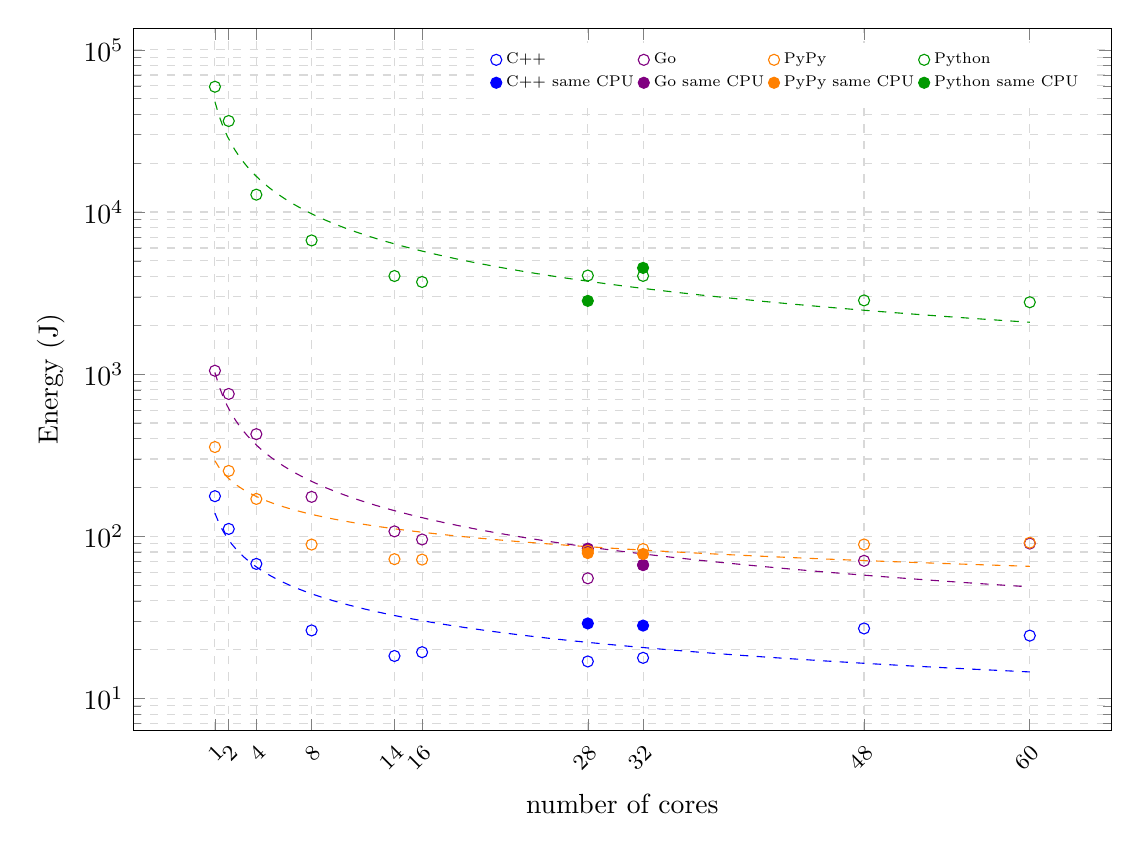
\begin{tikzpicture}
  \begin{semilogyaxis}[
      width=14cm,
      height=10.5cm,
      xlabel={number of cores},
      ylabel={Energy (J)},
      ymode=log,
      xmode=linear,
      grid=both,
      minor tick num=1,
      grid style={gray!30,dashed},
      xtick={1,2,4,8,14,16,28,32,48,60},
      x tick label style={
        font=\footnotesize,
        rotate=45,
        anchor=north east
      },
      legend style={
        at={(0.98,0.98)},
        anchor=north east,
        font=\scriptsize,
        nodes={scale=0.8,transform shape},
        draw=none
      },
      legend columns=2,
      transpose legend,
      legend cell align=left,
    ]

    %% C++ %%
    \addplot[
      blue,
      only marks,
      mark=o,
      mark options={draw=blue,fill=white}
    ] table[row sep=\\] {
      x    y \\
      1    176.83  \\
      2    111.08  \\
      4    67.60   \\
      8    26.28   \\
      14   18.28   \\
      16   19.29   \\
      28   16.91   \\
      32   17.80   \\
      48   27.02   \\
      60   24.40   \\
    };
    \addlegendentry{C++}
    \addplot[
      blue,
      only marks,
      mark=*,
      mark options={draw=blue,fill=blue}
    ] table[row sep=\\] {
      x    y \\
      28   29.01   \\
      32   28.15   \\
    };
    \addlegendentry{C++ same CPU}
    % power‐law fit: y = 138.9 * x^(–0.5506)
    \addplot[
      blue,
      dashed,
      forget plot,
      domain=1:60,
      samples=200
    ] {138.9 * x^(-0.5506)};

    %% Go %%
    \addplot[
      violet,
      only marks,
      mark=o,
      mark options={draw=violet,fill=white}
    ] table[row sep=\\] {
      x    y \\
      1    1049.92 \\
      2    755.43  \\
      4    426.69  \\
      8    175.15  \\
      14   107.26  \\
      16   95.60   \\
      28   55.07   \\
      32   66.51   \\
      48   70.64   \\
      60   90.23   \\
    };
    \addlegendentry{Go}
    \addplot[
      violet,
      only marks,
      mark=*,
      mark options={draw=violet,fill=violet}
    ] table[row sep=\\] {
      x    y \\
      28   83.98   \\
      32   66.54   \\
    };
    \addlegendentry{Go same CPU}
    % power‐law fit: y = 1024.9 * x^(–0.7437)
    \addplot[
      violet,
      dashed,
      forget plot,
      domain=1:60,
      samples=200
    ] {1024.9 * x^(-0.7437)};

    %% PyPy %%
    \addplot[
      orange,
      only marks,
      mark=o,
      mark options={draw=orange,fill=white}
    ] table[row sep=\\] {
      x    y \\
      1    355.42  \\
      2    253.06  \\
      4    170.08  \\
      8    88.94   \\
      14   72.28   \\
      16   71.84   \\
      28   81.44   \\
      32   83.50   \\
      48   89.06   \\
      60   91.31   \\
    };
    \addlegendentry{PyPy}
    \addplot[
      orange,
      only marks,
      mark=*,
      mark options={draw=orange,fill=orange}
    ] table[row sep=\\] {
      x    y \\
      28   78.81   \\
      32   77.79   \\
    };
    \addlegendentry{PyPy same CPU}
    % power‐law fit: y = 292.4 * x^(–0.3661)
    \addplot[
      orange,
      dashed,
      forget plot,
      domain=1:60,
      samples=200
    ] {292.4 * x^(-0.3661)};

    %% Python %%
    \addplot[
      green!60!black,
      only marks,
      mark=o,
      mark options={draw=green!60!black,fill=white}
    ] table[row sep=\\] {
      x    y \\
      1    59269.48 \\
      2    36442.43 \\
      4    12799.44 \\
      8    6683.08  \\
      14   4031.07  \\
      16   3705.32  \\
      28   4057.46  \\
      32   4037.98  \\
      48   2850.62  \\
      60   2777.96  \\
    };
    \addlegendentry{Python}
    \addplot[
      green!60!black,
      only marks,
      mark=*,
      mark options={draw=green!60!black,fill=green!60!black}
    ] table[row sep=\\] {
      x    y \\
      28   2831.52 \\
      32   4523.59 \\
    };
    \addlegendentry{Python same CPU}
    % power‐law fit: y = 4.79e4 * x^(–0.7649)
    \addplot[
      green!60!black,
      dashed,
      forget plot,
      domain=1:60,
      samples=200
    ] {4.79e4 * x^(-0.7649)};

  \end{semilogyaxis}
\end{tikzpicture}
\caption{Energy consumption of the server's \gls{ram} in Joules for different core configurations}
\label{fig:server-energy-ram}
\end{figure}


\begin{table}
    \centering
    \begin{tabular}{lrrrr}
        \hline
        energy-ram      & C++       & Go        & PyPy      & Python      \\
        \hline
        1               &   176.83  & 1,049.92  &   355.42  &  59,269.48  \\
        2               &   111.08  &   755.43  &   253.06  &  36,442.43  \\
        4               &    67.60  &   426.69  &   170.08  &  12,799.44  \\
        8	              &    26.28 	&   175.15  &    88.94  &	  6,683.08  \\
        14              &    18.28  &   107.26  &    72.28  &   4,031.07  \\
        16              &    19.29  &    95.60  &    71.84  &   3,705.32  \\
        28              &    16.91  &    55.07  &    81.44  &   4,057.46  \\
        28 same CPU     &    29.01  &    83.98  &    78.81  &   2,831.52  \\
        32              &    17.80  &    66.51  &    83.50  &   4,037.98  \\
        32 same CPU     &    28.15  &    66.54  &    77.79  &   4,523.59  \\
        48              &    27.02  &    70.64  &    89.06  &   2,850.62  \\
        60              &    24.40  &    90.23  &    91.31  &   2,777.96  \\
        \hline
    \end{tabular}
    \caption{Energy usage (RAM) by implementation and core count}
    \label{tab:server-energy-ram}
\end{table}